\documentclass[letterpaper,10pt]{article}

\usepackage{titling}
\usepackage{listings}
\usepackage{url}
\usepackage{setspace}
\usepackage{subfig}
\usepackage{sectsty}
\usepackage{pdfpages}
\usepackage{colortbl}
\usepackage{multirow}
\usepackage{multicol}
\usepackage{relsize}
\usepackage{amsmath}
\usepackage{fancyvrb}
\usepackage{amsmath,amssymb,amsthm,graphicx,xspace}
\usepackage[titlenotnumbered,noend,noline]{algorithm2e}
\usepackage[compact]{titlesec}
\usepackage{XCharter}
\usepackage[T1]{fontenc}
\usepackage{tikz}
\usetikzlibrary{arrows,automata,shapes,trees,matrix,chains,scopes,positioning,calc}
\tikzstyle{block} = [rectangle, draw, fill=blue!20, 
    text width=2.5em, text centered, rounded corners, minimum height=2em]
\tikzstyle{bw} = [rectangle, draw, fill=blue!20, 
    text width=4em, text centered, rounded corners, minimum height=2em]

\newcommand{\CPP}{C\nolinebreak\hspace{-.05em}\raisebox{.4ex}{\tiny\bf +}\nolinebreak\hspace{-.10em}\raisebox{.4ex}{\tiny\bf +}}
\def\CPP{{C\nolinebreak[4]\hspace{-.05em}\raisebox{.4ex}{\tiny\bf ++}}}

\let\LaTeXtitle\title
\renewcommand{\title}[1]{\LaTeXtitle{\textsf{#1}}}


\addtolength{\oddsidemargin}{-1.000in}
\addtolength{\evensidemargin}{-0.500in}
\addtolength{\textwidth}{2.0in}
\addtolength{\topmargin}{-1.000in}
\addtolength{\textheight}{1.75in}
\addtolength{\parskip}{\baselineskip}
\setlength{\parindent}{0in}
\renewcommand{\baselinestretch}{1.5}

\singlespace

\begin{document}

\lecture{ 6 --- Modern Processors}{\term}{Jeff Zarnett}

You know how \url{http://computers-are-fast.github.io/} featured in Lecture 1? It may also feature on your exams. You might want to print out you results and bring them.

\section*{Modern Processors}

It's critical to understand what's going on with the hardware if we want to write good programs. This lecture is based off the talk by Cliff Click~\cite{modern-hardware}.

Remember the classic von Neumann machine architecture. A program is comprised of both instructions and data, both of which are stored in the same memory. A program executes sequentially, one statement at a time, one after another. That is not really how computers work, at least not anymore, but it is an abstraction we still maybe find useful when it comes to algorithm analysis.

Consider this graph of CPU clock speed (frequency) over time from~\cite{cpudb}:

\begin{center}
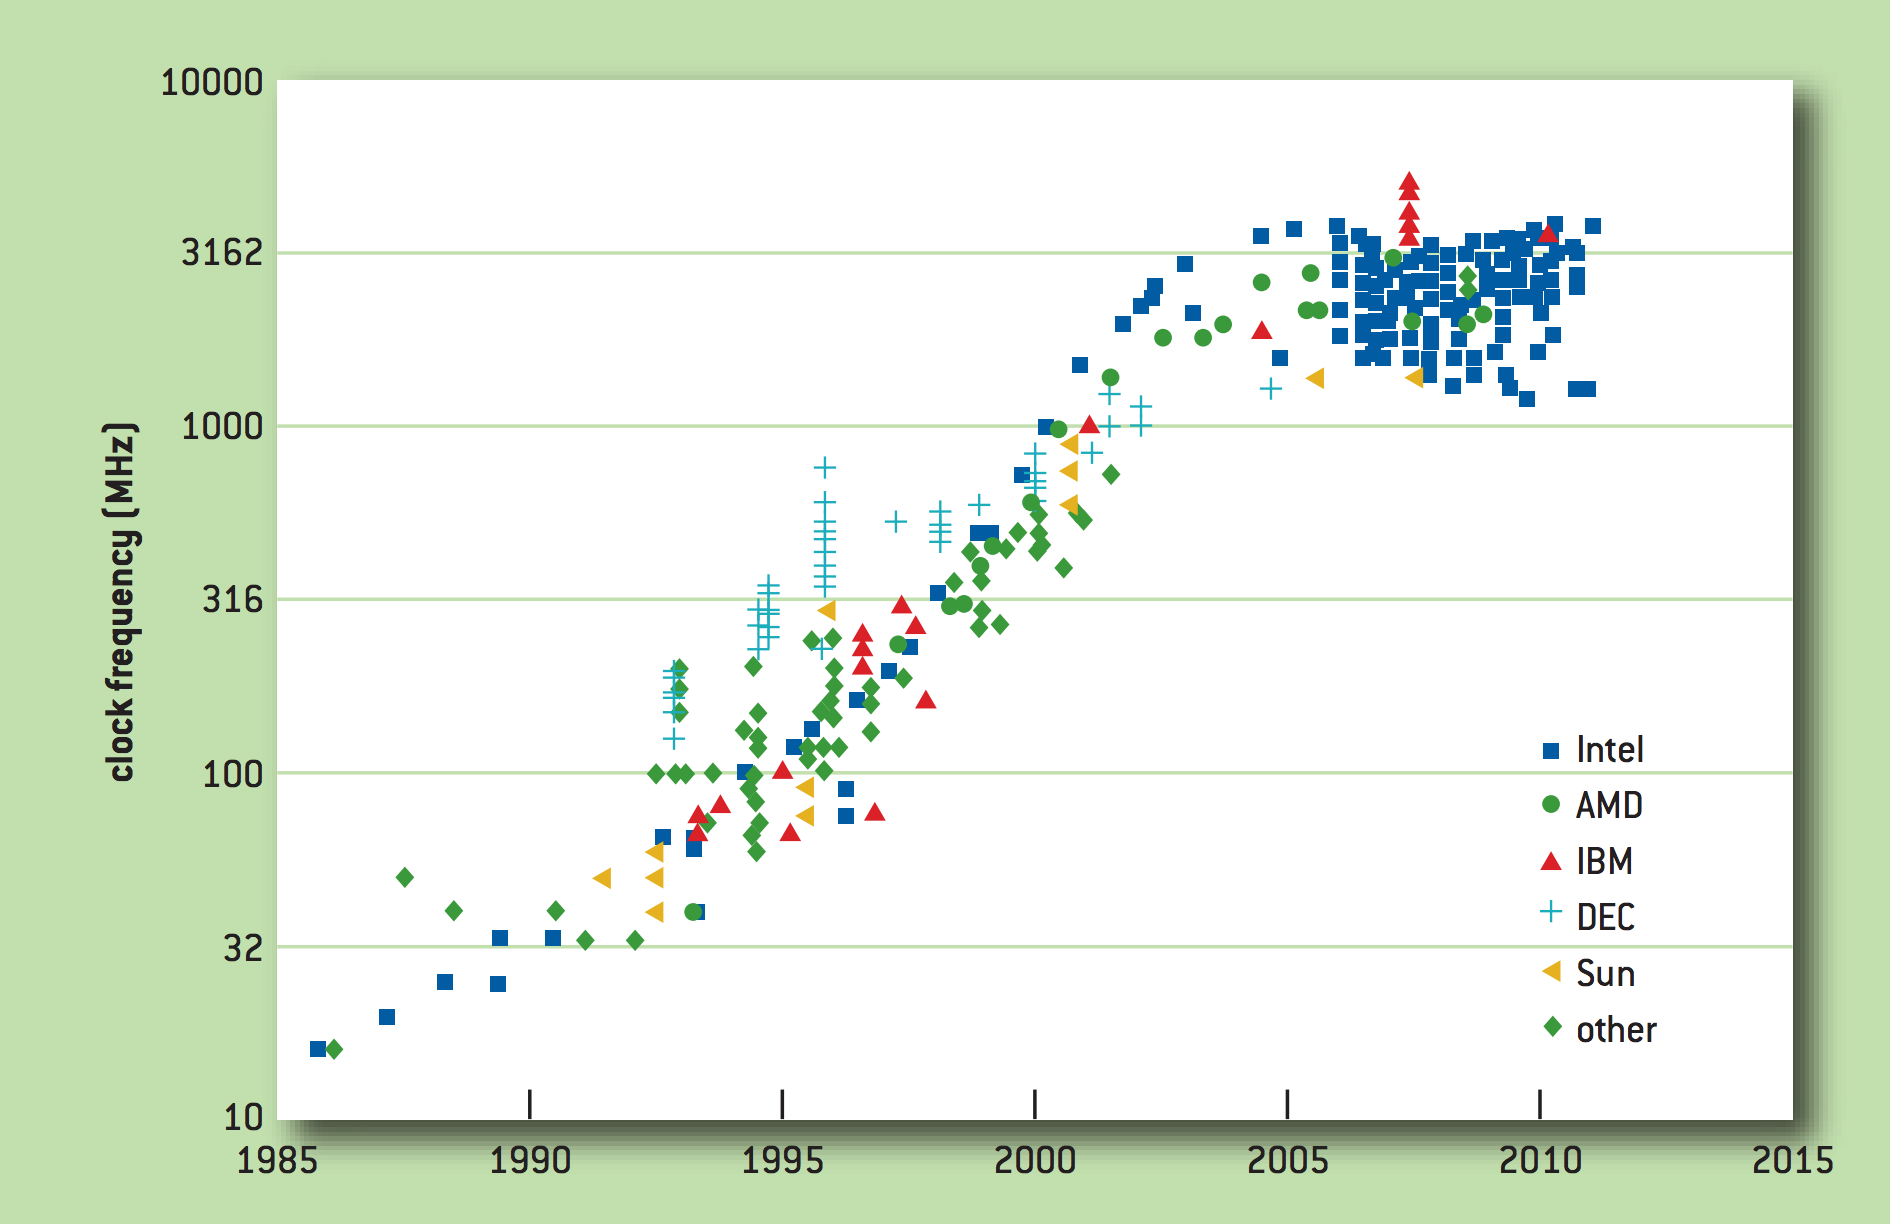
\includegraphics[width=0.7\textwidth]{images/cpu-frequency}
\end{center}

Clearly there is an area in which frequency scaling was effective. Next year's CPU would have a higher clock speed, and higher clock speed means more cycles per second, and more cycles per second means more work is done in a given second, and that means better performance. Except, we hit the wall: clock speeds stop getting faster around 2005, stopping at around 3 GHz. Speeding them up beyond this would take, well, more voltage which means more power and more heat, and more heat means higher failure/error rates, and more cooling, and the cooling takes power too, and all that waste heat, well, it will eventually, at the end of this chain, make polar bears sad.

Digression: if we look at the x86 processor, one with which everyone is probably at least \textit{passingly} familiar, it is a Complex Instruction Set Computing (CISC) processor. In other words, there are a lot of assembly instructions. But why? This was intended for your convenience as a programmer: if you were going to write assembly, wouldn't it be nice to have a sine function that takes one argument instead of having to grind out (or copy-paste) the calculation of a sine routine every single time you needed it? So the hardware people thought they were doing everyone a favour. These are easy to program in, from the way the assembly programmer thinks, but hard to implement and hard to pipeline. 

For a lot of CISC machines, the Cycles Per Instruction (CPI) varied, something like 4-10 cycles to complete any instruction, but at least it was predictable. Every time, no matter what, it takes the same number of cycles. Program performance was basically the number of page faults (disk accesses) times the amount of time it takes to read from disk, plus the instruction execution time (which is generally small compared to page fault service times)\footnote{For further discussion about this, see the ECE~254 notes about page faults and caching and disk read times.}. Thus the optimization goal is: minimize page faults. Page fault count is relatively easy to measure and there are some things we can do to reduce the number of page faults; optimize our data access patterns, change how we pack the data, et cetera. If you were working with an embedded system with no disk (or at least no page faults) then the optimization goal is minimize instruction count.

Between 1990 and 2005 we got some really impressive scaling on CPU frequency. This was caused by a few factors. The first is the advent of the Reduced Instruction Set Computing (RISC) CPU: simpler processors are easier to scale than complex ones, and simpler instructions mean fewer cycles per instruction. That also means we can have more pipelining. The tradeoff is that RISC CPUs are much harder to program in assembly directly, so compilers had to do the work. The example in~\cite{modern-hardware} is delay slots: an instruction after a branch is always executed or worse, the result of a computation is not available to the next instruction. In these cases the ``simple'' solution is to put a \texttt{NOP} (do-nothing) instruction in, good compilers (and programmers) can rearrange instructions, hopefully, to make this work without wasting time. And another thing: memory got cheaper, so we have more of it, so page faults occurred less and less frequently and that's really something.

But then, as we have seen, we hit the (power) wall. And you might think, well, if I run into a wall, I can just go around it. There must be other ways to advance! And there are, except, we hit three other walls too, and now we are surrounded\footnote{``He is intelligent, but not experienced. His pattern indicates two dimensional thinking.'' - Spock, \textit{Star Trek II: The Wrath of Khan}}. What are these other three seemingly-insurmountable barriers?

The first is instruction level parallelism (ILP) is getting close to the limit of what we can do. We can predict branches with a certain accuracy but if we have already got 95\% efficiency, no matter how much time and effort and money is invested into improving the branch prediction routine we get maximally a 5\% increase in branch prediction accuracy which translates into a very small speedup to the execution when we consider just how often a misprediction is the cause of the problem (5\% of 5\% is very small\ldots just making up numbers).

The speed of memory advances has not at all kept up with the advances in CPU technology, so now we have moved from the era of runtime being dominated by page faults to the era of runtime being dominated by cache misses. Adding more cache isn't a perfect solution though, and doubling, say, level one cache (at great expense) does not double the speed of the program; it may speed it up by a small amount at most. 

The final wall is the universal speed limit: the speed of light (curse you Einstein!). The more complex the CPU is, the longer the path any signal may have to travel to get from A to B. This is limited, most practically, by the speed of light, and thus far, nobody has invented a way to get around this universal speed limit (but we are working on it, and according to Star Trek, should have this sorted out by 2063 or so).

But let's go back to the subject of ILP. Branch prediction and pipelining have been touched upon but there is so much more to it. The idea with ILP is not having more cycles to work with, but instead, doing more in each clock cycle. And there's a lot of clever ideas. 

Pipelining: you may have heard a bit about this already, especially so if you have taken a CPU architecture course. To complete an instruction there are five basic steps: (1) fetch the instruction from memory, (2) decode the instruction, (3) fetch needed operands, (4) perform the operation, and (5) write the result. So to do an instruction like \texttt{ADD R1, R2}, we need to fetch the instruction, decode it and figure out what is to be done, read the values from \texttt{R1} and \texttt{R2}, do the addition, and then write the result to \texttt{R1}. Thus even a simple instruction takes more than one clock cycle, but the good news is that the stages can overlap:

\begin{center}
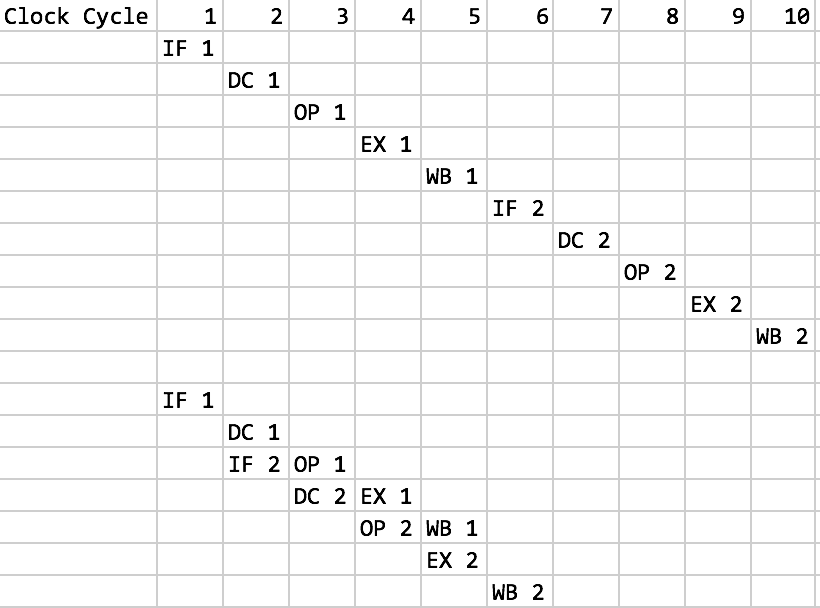
\includegraphics[width=0.4\textwidth]{images/pipelining}
\end{center}

In the above image, two instructions are shown. The top part shows no pipelining; the bottom shows what happens when pipelining is used. Each part of the instruction must be done sequentially---the instruction cannot be decoded until it is fetched---but at least the next instruction can be done. So it allows each of these to appear as if it is 1 clock cycle. If all goes well, then you complete one instruction per clock cycle. 

But there are pipeline hazards: sometimes you need the result of a previous step before you can go on. These prevent us from reaching the theoretical maximum of one instruction completed per clock cycle. Needing a previous result is not the only kind of hazard, though; we may have conflicts over certain CPU resources (how many floating point units are there, after all\ldots?) or fetch may be unable to identify the next instruction because of a branch. In the worst case, if we have mispredicted a branch, we have to flush the pipeline: throw away the instructions fetched, decoded, operands prepared, et cetera, because we guessed wrong and started doing the wrong actions. In that case, some extra work was done that was not necessary\ldots

The next idea relates to getting items from memory. If we do a load from memory, and we are lucky, it is found in the fastest cache and is available in perhaps 2-3 clock cycles. If we must go to memory, it may be 200-300 cycles. If it is in level 2 or level 3 cache it will be somewhere in between. The key idea, though, is if we are trying to put something in register \texttt{R7}, it will take time until that value is actually present in that register. The simplest approach is to just wait around until that value has arrived, and then go on to the next instruction. That works, but we can do better.

That better idea is: continue executing until \texttt{R7} is used somewhere. This allows us to get some useful work done in the meantime. Hardware keeps track of the fact that the register is not quite ready yet, but the work can get done in what is called the ``miss shadow''. It's possible to have more than one load in flight at a time. Two or more can be done in various CPU architectures, but it is of course hardware dependant. 

Branch prediction has come up already, but if we have a load followed by a compare used as a branch, we can then, well, guess. If we are wrong, there is the need to cleanup. But the good news is that branch prediction is usually right most of the time, perhaps 95\% or more (we'll definitely return to this later).

Another nice thing that the hardware can do for us is ``dual issue'' instructions. If we have two consecutive instructions that both take the same amount of time, use unrelated registers, and don't consume two of the same resource, we can start both instructions at once. If the instructions are \texttt{ADD R1, 16} and \texttt{CMP R2, 0} they do different things with different registers so there is no reason these cannot be done in parallel (if there are enough fetch/decode/etc units). In an embedded system, you may be interested in ensuring that this happens during a computationally intensive loop, such as encoding/decoding of media. If programmed correctly, you can be sure you get dual issue on every cycle.

Then a group of things that somewhat go together: register renaming, branch prediction, speculation, and Out-of-Order (O-O-O) Execution. These all work synergistically: each adds to the benefits the other brings. Register renaming works on a fairly simple principle: an assembly instruction says to read from register \texttt{R4}, but behind the scenes inside the processor, it is mapped to a physical register (let's say \texttt{RA} for the purpose of the example). Consider the following assembly instructions:

\begin{verbatim}
MOV R2, R7 + 32
ADD R1, R2
MOV R2, R9 + 64
ADD R3, R2
\end{verbatim}

Under normal circumstances, we cannot do instruction 3 until instruction 2 has been completed because we need the value of \texttt{R2} that was put in there (taken from memory somewhere) to be added to \texttt{R1}. Except, with register renaming, behind the scenes the first two instructions may replace \texttt{R2} with \texttt{RX} and the second pair of instructions have \texttt{R2} replaced with \texttt{RY} and these things can take place in parallel, or without a stall, at the very least.

This has a certain synergy with branch prediction. If we predict a branch, we can do speculative changes into one set of registers while we keep the ``old'' register values around too. When we figure out whether the branch prediction is correct, we can then get rid of the ones we don't need: the originals if predicted correctly, and the new values otherwise. So we get better recovery if there is a misprediction. Actually, I bet students wish they could do this: write down both answers to a question and let the TA pick the correct one at the end\ldots

Most importantly, it allows us to get past a cache miss and keep going; the goal here is to run until we can start the next cache miss, because the sooner that starts the sooner it's over, and the faster the program executes, ultimately. A quick example from the presentation demonstrates this, in x86 assembly~\cite{modern-hardware}:

\begin{verbatim}
ld rax, rbx+16   ; assume cache miss
add rbx, 16      ; carry on anyway, ADD doesn't need rax value from LD
                 ; register renaming => LD (write)/ADD (read) don't interfere
cmp rax, 0       ; needs rax value, queue till available
jeq null_chk     ; oops! need cmp result
                 ; speculate: assume branch not taken
st rbx-16, rcx   ; speculatively store to store buf (not L1)
ld rcx, rdx      ; unrelated cache miss: 2 misses now active, 1 speculative
ld rax, rax+8    ; now must wait for result of first LD
\end{verbatim}

%Let's assume \texttt{rax} (register A) is not available and the first instruction is a cache miss and it will take 300 cycles to get it. So we carry on. Then the instruction next is unrelated so we can go on. It doesn't matter that \texttt{rbx} is read in the first two instructions, because we can do register renaming so that internally it's reading from register 4 and writing to register 12. The compare cannot proceed because the first load's value is not available, but it will be queued up to be done later. Then we have a branch, but we don't know what the flags are, because we can't compare, because the load isn't done. The branch predictor will say in this example that we will not take the branch and go on to the store instruction (\texttt{st}). The store is speculative because the branch may have been taken (so it goes in a store buffer temporarily and not to L1 cache, until we are sure it's okay to let it go to memory). We have now made it to the second last line and we have another unrelated cache miss, and we have two cache misses running in parallel (the second of which is speculative). Finally, the last instruction has to wait for the first instruction to fill the register \texttt{rax} and we can no longer speculate.

To summarize: there are seven operations we were trying to do here with two cache misses. The cache misses complete in cycles 300 and 304 (maybe 302 if we have dual issue), so in total we complete 7 operations in about 305 cycles. All the trickery and cleverness got us to that second miss which means we complete in 305. If we did not manage that, it would take about 600 cycles to complete it all. So we did double performance, even though in this example our overall performance was terrible.
 
For years Intel was trying to push its Itanium processors (which were so unsuccessful they got the nickname ``Itanic''. Ouch). The goal of these was to find static (compile-time) parallelism: if a machine has infinite registers, can speculate infinitely, etc, the program gets sped up. Run all possibilities in parallel and at the end figure out which is right (wasn't this a Nicolas Cage movie?). Unfortunately it didn't work out very well because this requires the right kind of program and an super smart compiler. Oh yes, and infinite registers requires infinite space as well as infinite money. So instead the quest has turned to how we can get better performance out of x86\ldots

The x86 approach tries to maximize dynamic (run-time) parallelism. This has been done incrementally, with more pipelining, re-order buffers, adding more functional units, and so on. But the walls are still there: cache miss rates and branch mispredicts continue to dominate performance, even though the rates are very low, because a miss costs so much. 

How are we doing so far? Well, here's a short video that goes over where we were in the beginning of 2017: \url{https://www.youtube.com/watch?v=4A0Iks4ENIs} with the launch of Intel's latest (at the time) processor. But since then, AMD launched Ryzen---Never turn your back on Threadripper!---and it's forced Intel to compete again\ldots In 2020 the situation is more like \url{https://www.youtube.com/watch?v=a8apEJ5Zt2s}.

According to~\cite{modern-hardware} something like 90-99\% of the transistors on a modern x86 chip are spent in cache. In spite of the extreme complexity of the decode logic that allows multiple parallel decodes of all the weird and wacky instructions of the x86, pushing cache to the biggest size it can be is so important because it prevents the performance hit of going to memory.

The image below (from Sun World Wide Analyst Conference in 2003) is obviously a bit dated but this is very instructive as to the trend:
\begin{center}
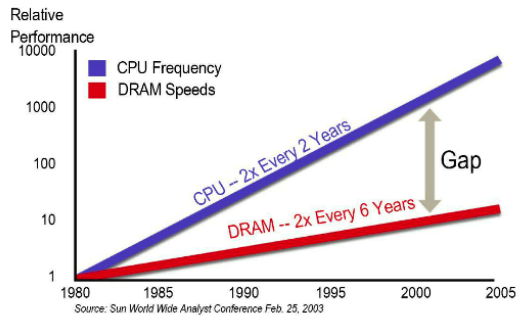
\includegraphics[width=0.6\textwidth]{images/ram-vs-cpu.png}
\end{center}

DRAM is, however, not the only kind of memory. There is SRAM (Static RAM) which is fast but expensive, the kind of stuff that goes on the CPU die, and it is six transistors per bit. Compare against DRAM which is much cheaper, but slow: one transistor and one capacitor per bit. Improvements in DRAM have not really improved latency but have improved bandwidth; DDR (Dual Data Rate\ldots not Dance Dance Revolution) means there are two transfers per cycle, but it still takes significant time to get any data out. And DRAM needs occasional refreshes (capacitors\ldots) so sometimes we have to wait for that.

In the Operating Systems course you probably learned that disk is the slowest thing and the limiting factor. That's true, as Obi-Wan Kenobi would say, from a certain point of view. Now that we live in the world of Solid State Drives (SSDs), ``disk'' reads are about as fast as memory reads and memory reads are the rate-limiting step in the system. Nonvolatile memory looks to be even faster. More is the new more, orange is the new black, and memory is the new disk.

To get memory access speed up there are things we can do, like relax coherency constraints, more synchronization through locks\ldots all of which we will come back to in some upcoming lectures. 

If we want to get better performance, we need to figure out where time is going. For that we will have the subject of profiling, which comes up in some later lectures. If we can track down where our cache misses are occurring, maybe, just maybe, we can do something about it. 

\section*{A Deeper Look at Cache Misses}

As discussed, the CPU generates a memory address for a read or write operation. The address will be mapped to a page. Ideally, the page is found in the cache, because that would be faster. If the requested page is, in fact,  in the cache, we call that a cache \textit{hit}. If the page is not found in the cache, it is considered a cache \textit{miss}. In case of a miss, we must load the page from memory, a comparatively slow operation. The percentage of the time that a page is found in the cache is called the \textit{hit ratio}, because it is how often we have a cache hit. We can calculate the effective access time if we have a good estimate of the hit ratio (which is not overly difficult to obtain) and some measurements of how long it takes to load data from the cache and how long from memory. The effective access time is therefore computed as:

\begin{center}
Effective Access Time = $h \times t_{c} + (1-h) \times t_{m}$
\end{center}

Where $h$ is the hit ratio, $t_{c}$ is the time required to load a page from cache, and $t_{m}$ is the time to load a page from memory. Of course, we would like the hit ratio to be as high as possible. 

Caches have limited size, because faster caches are more expensive. With infinite money we might put everything in registers, but that is rather unrealistic. Caches for memory are very often multileveled; Intel 64-bit CPUs tend to have L1, L2, and L3 caches. L1 is the smallest and L3 is the largest. Obviously, the effective access time formula needs to be updated and expanded when we have multiple levels of cache with different access times and hit rates. See the diagram below:

\begin{center}
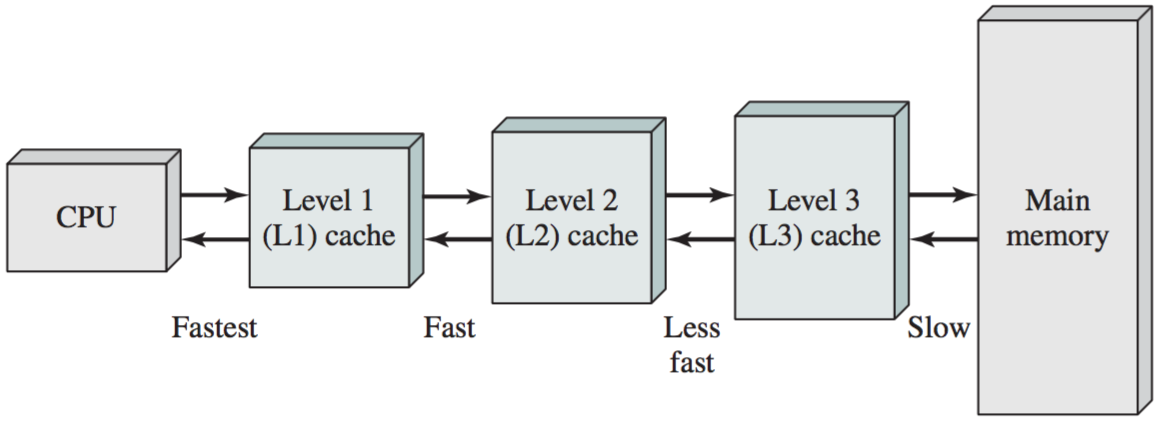
\includegraphics[width=0.6\textwidth]{images/caches.png}\\
Three levels of cache between the CPU and main memory~\cite{osi}.
\end{center}

If we have a miss in the L1 cache, the L2 cache is checked. If the L2 cache contains the desired page, it will be copied to the L1 cache and sent to the CPU. If it is not in L2, then L3 is checked. If it is not there either, it is in main memory and will be retrieved from there and copied to the in-between levels on its way to the CPU. 

Cliff Click said that 5\% miss rates dominate performance. Let's look at why.
I looked up a characterization of the SPEC CPU2000 and CPU2006 
benchmarks~\cite{cpu2006}.

Here are the reported cache miss rates\footnote{\permil~is ``permil'', or per-1000.} for SPEC CPU2006.

\begin{center}
\begin{tabular}{ll}
L1D & 40\permil \\
L2 & 4 \permil
\end{tabular}
\end{center}

Let's assume that the L1D cache miss penalty is 5 cycles and the L2 miss penalty is
300 cycles, as in the video. Then, for every instruction, you would expect a running
time of, on average:
\[ 1 + 0.04 \times 5 + 0.004 \times 300 = 2.4. \]
Misses are expensive!


If we replace the terms $t_{c}$ and $t_{m}$ with $t_{m}$ and $t_{d}$ (time to retrieve it from disk) respectively, and redefine $h$ as $p$, the chance that a page is in memory, we can get an idea of the effective access time in virtual memory: 

\begin{center}
	Effective Access Time = $ p \times t_{m} + (1 - p) \times t_{d}$
\end{center}

And just while we're at it, we can combine the caching and disk read formulae to get the true effective access time for a system where there is only one level of cache:

\begin{center}
	Effective Access Time = $ h \times t_{c} + (1 - h) ( p \times t_{m} + (1 - p) \times t_{d})$
\end{center}

This is good, but what is $t_{d}$? This is a measurable quantity so it is possible, of course, to just measure it\footnote{One of my favourite engineering sayings is ``Don't guess; measure.'' You may be sick of hearing me say that one by now.}.

The slow step in all of this, is obviously, the amount of time it takes to load the page from disk. According to~\cite{osc}, restarting the process and managing memory and such take something like 1 to 100~$\mu$s. A typical hard drive in their example has a latency of 3~ms, seek time (moving the read head of the disk to the location of the page) is around 5~ms, and a transfer time of 0.05~ms. So the latency plus seek time is the limiting component, and it's several orders of magnitude larger than any of the other costs in the system. And this is for servicing a request; don't forget that several requests may be queued, making the time even longer.

Thus the disk read term $t_{d}$ dominates the effective access time equation. If memory access takes 200~ns and a disk read 8~ms, we can roughly estimate the access time in nanoseconds as $(1-p) \times 8~000~000$. 

If the page fault rate is high, performance is awful. If performance of the computer is to be reasonable, the page fault rate has to be very, very low.

Summary: misses are not just expensive, they hurt performance more than anything else.

\bibliographystyle{alphaurl}
\bibliography{459}



\end{document}
